\documentclass{standalone}

\usepackage{graphicx}
\usepackage{color}
\usepackage{tikz}
\usepackage{pgfplots}
\usepackage{pgf-umlsd}
\usepackage{ifthen}

\usetikzlibrary{positioning,calc}


%%%%%%%%%%%%
%Figure adapted from: He, Kaiming, Xiangyu Zhang, Shaoqing Ren, and Jian Sun. "Deep residual learning for image recognition." In Proceedings of the IEEE conference on computer vision and pattern recognition, pp. 770-778. 2016.
%%%%%%%%%%%%

\pgfplotsset{compat=1.16} 

\begin{document}


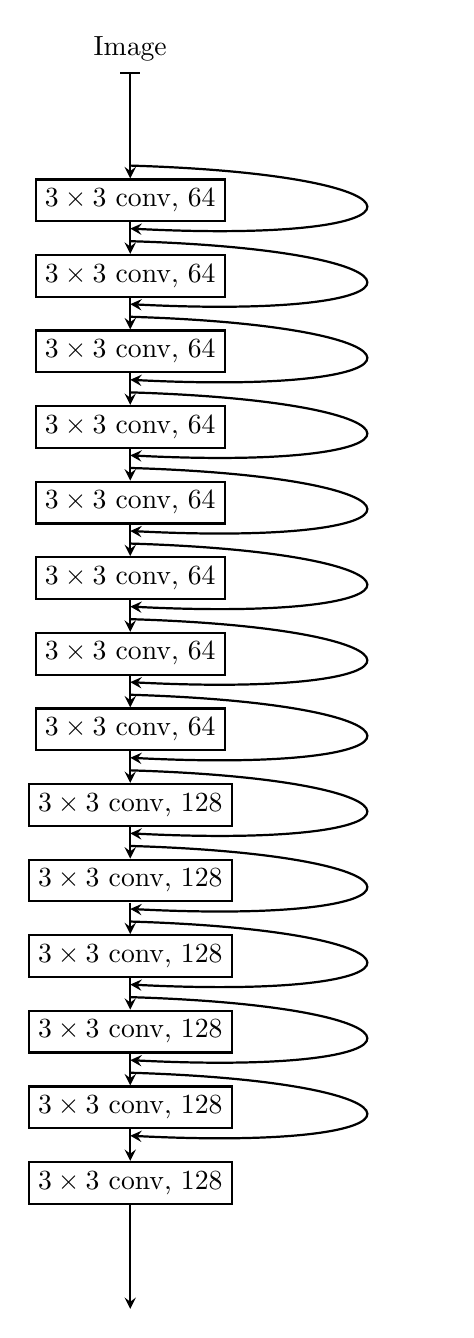
\begin{tikzpicture}[scale=0.8, -stealth, thick]
\path (0, 0) node[rectangle] (img) {Image};
\foreach \na / \y in {2,...,9}
    \path (0, -1.2*\y) node[draw, rectangle] (I-\na) {$3\times 3$ conv, 64};
\foreach \na / \y in {10,...,15}
    \path (0, -1.2*\y) node[draw, rectangle] (I-\na) {$3\times 3$ conv, 128};

\draw[|-stealth] (img)--(I-2);
\draw[-stealth] (I-15)--++(0, -2);
\foreach \y in {2,...,14}{
    \draw (I-\y) -- ++(0, -0.85);
};

% \foreach \y/\z in {2/3,13/14}{
%     \draw (I-\y) -- (I-\z);
% };

\foreach \y in {2,...,14}{
    \draw (I-\y)++(0, 0.55) .. controls +(5cm, -0.15) and +(5cm, -0.25).. ++(0, -1);
};
\end{tikzpicture}


\end{document}